En este capítulo se detalla cada uno de los puntos llevados a cabo para la realización de este proyecto, empezando por definir la propuesta realizada, luego explicar el proceso ingenieril llevado a cabo y terminar desglosando el trazado de la ejecución de este proyecto.

\section{Propuesta}

El trabajo propuesto tiene como objetivo la creación de un elemento software funcional que, usando el paradigma lógico explicado en la sección \ref{asp}, permita la generación de un escenario jugable que pueda ser ejecutado en el juego Freeciv [ver sección \ref{subsec:freeciv}]. Así mismo incluirá una interfaz gráfica interactuable que permitan al usuario marcar que zonas del terreno deben generarse y cuales no, indicando su contenido antes de lanzar el proceso de generación.

\subsection{Formato del escenario de Freeciv}

Como uno de los puntos fuerte de este trabajo tiene que ver con la generación de escenarios, este sistema tiene que tener como salida un mapa válido que sea leído correctamente por el juego Freeciv. Es por eso que explicaré en detalle el formato usado. \\

Para empezar, el formato se basa en archivo de texto plano que contiene varios campos, haciendo que sea lo más simple posible y que en la teoría se pueda modificar a mano.

\begin{lstlisting}[caption=Ejemplo de formato de mapa]
[settings]
set={"name","value","gamestart"
     "mapsize","FULLSIZE","FULLSIZE"
     "size",0,0
     "tilesperplayer",100,100
     "xsize",16,16
     "ysize",16,16
     "topology","WRAPX|WRAPY","WRAPX|WRAPY"
     [...]
}

[map]
have_huts=FALSE
t0000="h+hf  aaaa    ff"
t0001="dgg    aat    ff"
t0002="hhh           pp"
t0003="hmp        ggghh"
t0004="hmh       s dghf"
t0005=" dg      phffpm "
t0006="                "
t0007="aa     sdg    aa"
t0008="aa      h     aa"
t0009="       jff p    "
t0010="mh      s pdp pm"
t0011="gf       pdhh   "
t0012="        gpsg   p"
t0013="      h  hh     "
t0014="hff         gg s"
t0015="m+h   aaaa   m f"
startpos_count=5
startpos={"x","y","exclude","nations"
          0,2,FALSE,""
          9,11,FALSE,""
          14,0,FALSE,""
          2,5,FALSE,""
          12,3,FALSE,""
}
b00_0000="0000000000000000"
[...]
spe00_0000="0000000000000000"
[...]
spe01_0000="0000000000000088"
[...]
spe02_0000="0000000000000000"
[...]
res0000="c c   x i y  v  "
[...]
owner0000="3,3,3,3,-,-,-,-,-,-,-,-,-,-,-,3"
[...]
source0000="242,242,242,242,-,-,-,-,-,-,-,-,-,-,-,242"
[...]
worked0000="-,-,-,-,-,-,-,-,-,-,-,-,-,-,-,-,"
k00_0000="a88880000000222a"
[...]
k01_0000="0000000000000000"
[...]
k02_0000="0000000000000000"
[...]
k03_0000="0000000000000000"
[...]
k04_0000="0000000000000000"
[...]
k05_0000="0000000000000000"
[...]
k06_0000="0000000000000000"
[...]
k07_0000="0000000000000000"
[...]
\end{lstlisting}

El mapa es siempre una rejilla de dos dimensiones en el que cada celda es una baldosa o \textit{tile}. Esta rejilla puede estar configurada de varias maneras según su topología:

\begin{itemize}
	\item \texttt{warpx}: La topología de escenario es como un mapa terrestre, es decir el eje Este-Oeste se junta.
	\item \texttt{warpy}: La topología del escenario junta el eje Norte-Sur.
	\item \texttt{warpx warpy}: La topología del escenario es un toroide, es decir, tiene forma de donuts.
	\item \texttt{iso}: La rejilla del escenario es isométrico.
	\item \texttt{hex}: La rejilla del escenario es hexagonal.
	\item \texttt{iso hex}: La rejilla del escenario es en forma de panel de abeja.
\end{itemize}

Por otra parte, cada celda de la rejilla contendrá una baldosa de terreno único, que viene definido por un identificador único, el cual puede ser uno de los siguientes:

\def\arraystretch{1.5}%  1 is the default, change whatever you need

\begin{table}[h]
	\begin{tabular}{ p{0.7\textwidth} c c }
		\bfseries{Descripción} & \bfseries{ID} & \bfseries{Imagen} \\
		\hline
		\textit{Pradera}: Es uno de los terrenos más comunes. Las unidades se pueden mover fácilmente. & \texttt{g} & \adjustimage{height=2em,valign=t}{images/grassland.png} \\
		\textit{Llanura}: Es otro terreno muy común. Se puede usar para crear carreteras. & \texttt{p} & \adjustimage{height=2em,valign=t}{images/plains.png} \\
		\textit{Colinas}: Las unidades se mueven lentamente. Es uno de los terrenos con mayor bonus defensivo (200\%). & \texttt{h} & \adjustimage{height=2em,valign=t}{images/hills.png} \\
	\end{tabular}
	\caption{Tipos de terreno}\label{table:terrains1}
\end{table}

\begin{table}
	\begin{tabular}{ p{0.7\textwidth} c c }
		\bfseries{Descripción} & \bfseries{ID} & \bfseries{Imagen} \\
		\hline
		\textit{Bosque}: Produce una unidad de producción (madera) con la que construir edificaciones. Tiene un bonus defensivo de 150\% & \texttt{f} & \adjustimage{height=2em,valign=t}{images/forest.png} \\
		\textit{Jungla}: Puede llegar a producir 4 unidades de producción si se encuentran con recursos de gemas o fruta. & \texttt{j} & \adjustimage{height=2em,valign=t}{images/jungle.png} \\
		\textit{Montanas}: Es el terreno con mayor bonus defensivo (300\%). Solo las unidades aéreas (aviones, cazas, etc) pueden atravesarla. & \texttt{m} & \adjustimage{height=2em,valign=t}{images/mountains.png} \\
		\textit{Desierto}: Normalmente solo se puede usar para crear carreteras, pero si hay un modificador de oasis puede generar hasta 3 unidades de producción. & \texttt{d} & \adjustimage{height=2em,valign=t}{images/desert.png} \\
		\textit{Pantano}: Se puede irrigar rápidamente. Puede producir de 5 a 9 unidades de producción si se encuentra con recursos como tundra o con especias. & \texttt{s} & \adjustimage{height=2em,valign=t}{images/swamp.png} \\
		\textit{Tundra}: Solo se pueden crear carreteras. & \texttt{t} & \adjustimage{height=2em,valign=t}{images/tundra.png} \\
		\textit{Glacier}: Ninguna de las unidades puede cruzarlo. & \texttt{a} & \adjustimage{height=2em,valign=t}{images/glacier.png} \\
		\textit{Mar}: Todas las unidades acuáticas pueden cruzarlo. Puede producir 2 unidades de producción si se encuentra con un banco de peces & & \adjustimage{height=2em,valign=t}{images/sea.png} \\
		\textit{Océano}: Solo las grandes embarcaciones y submarinos pueden pasar por encima. & \texttt{:} & \adjustimage{height=2em,valign=t}{images/ocean.png} \\
	\end{tabular}
	\caption{Tipos de terreno}\label{table:terrains2}
\end{table}

\section{Proceso de ingeniería}

\subsection{Metodología}

\subsection{Gestión del proyecto}

\section{Análisis del software}

Una vez definido el sistema y planificada su construcción, se ha realizado un análisis en donde se identifican los requisitos que debe cumplir el software una vez terminado el proyecto.

\subsection{Requisitos funcionales}

Los requisitos funcionales son aquellas condiciones indispensables que estipulan las funcionalidades que debe proporcional el sistema. Para este proyecto se ha recogido los diferentes requisitos:

\begin{itemize}
	\item Generación de un mapa que sea legible por el videojuego Freeciv.
	\item Permitir añadir restricciones sobre ciertas zonas del mapa.
	\item Poder guardar y recuperar el mapa en un formato sencillo.
\end{itemize}

\subsection{Requisitos no funcionales}

Los requisitos no funcionales, por su contra, son aquellas condiciones indispensables que debe cumplir el sistema a la hora de diseñar e implementar. Para este proyecto se han tenido en cuenta estos requisitos:

\begin{itemize}
	\item Eficiencia y eficacia: El generador debe responder en el menor tiempo posible arrojando una respuesta óptima.
	\item Escalabilidad: El generador debe trabajar con mapas de diferentes tamaños, por lo que el sistema debe poder soportar cualquier tamaño de entrada.
	\item Usabilidad: La interfaz gráfica debe ser lo más sencilla posible, evitando que el usuario tenga que realizar tareas tediosas a la hora de construir mapas.
\end{itemize}

\section{Diseño del sistema}

Una vez definidos los requisitos se ha procedido a realizar el diseño software del sistema en cuestión, empezando a concretar la arquitectura propuesta y luego desenvolviendo los casos de uso y diagramas de clases.

\subsection{Arquitectura software}

Debido a que el sistema cuenta con una interfaz gráfica y un módulo que se encargará de generar el mapa, el sistema estará dividido en dos partes concretas tal y como se puede ver en la Figura \ref{fig:arquitectura}:

\begin{itemize}
	\item Una parte que será la aplicación gráfica, el cual sigue la estructura Modelo-Vista-Controlador (MVC). El controlador se encargará de hacer de puente entre la interfaz gráfica, que es lo que manipulará el usuario, y los datos guardados en memoria. Así mismo proporcionará las funcionalidades básicas del sistema como guardar o cargar el mapa y crear un mapa en blanco.
	\item La otra parte es el programa ASP que ejecutará Clingo. Contiene un controlador que se encargará de hacer la llamada a Clingo y de obtener su resultado, y luego otro controlador que se encargará de llamar primeramente al programa que genere las regiones y luego, dada una región, genere las casillas de la región.
\end{itemize}

Tanto el controlador de la interfaz de usuario como el controlador del programa ASP se ejecutarán en paralelo, pudiendo enviarse información de un controlador a otro para saber cuando hay que empezar una generación o si esta terminó. A pesar de esto, los resultados de la generación de ASP se guadarán en un archivo intermedio para evitar enviar gran cantidad de datos entre los elementos.

\begin{figure}
	\centering
	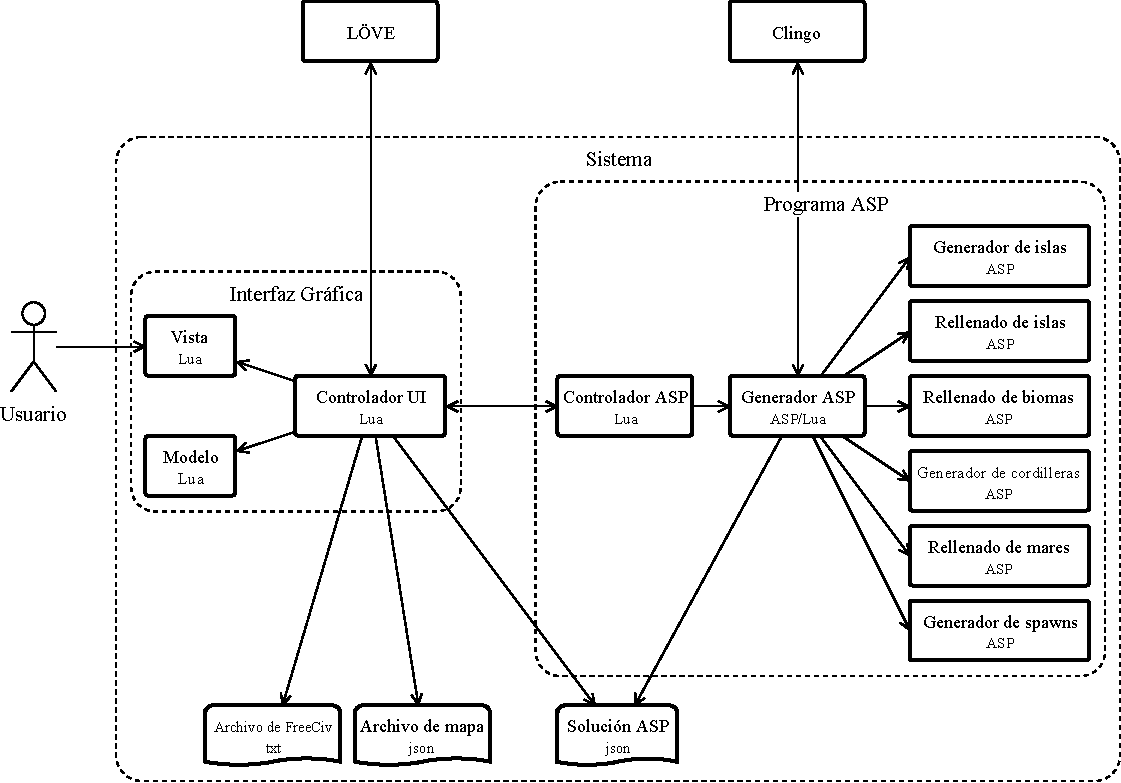
\includegraphics[height=10em]{images/arquitectura.pdf}
	\caption{Arquitectura del sistema}
	\label{fig:arquitectura}
\end{figure}

\subsection{Casos de uso}

\subsection{Implementación}